\documentclass[tikz,border=2pt]{standalone}
\usepackage{amsmath}
\usepackage{pgfplots}
\pgfplotsset{compat=1.18}
\usetikzlibrary{arrows.meta}
\begin{document}
% X = 1 surely, Y in {0,2} with probability 1/2 each (both means 1): F_Y = 1/2 >= F_X = 0 on [0,1),
% F_Y = 1/2 <= F_X = 1 on [1,2), equal from 2 on; one crossing at t_0 = 1, and the two gaps both have area 1/2.
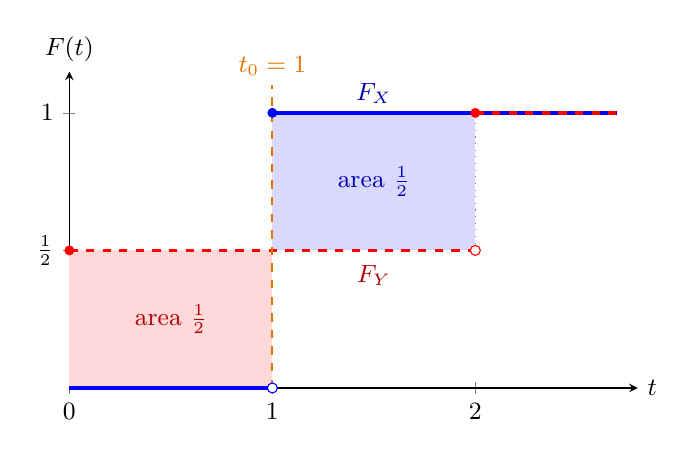
\begin{tikzpicture}[font=\small, >={Latex[length=2mm]}]
  \begin{axis}[
    axis lines=left, xmin=0, xmax=2.8, ymin=0, ymax=1.15,
    xtick={0,1,2}, ytick={0.5,1}, yticklabels={$\tfrac12$,$1$},
    xlabel={$t$}, ylabel={$F(t)$},
    xlabel style={at={(axis description cs:1,0)}, anchor=west},
    ylabel style={rotate=-90, at={(axis description cs:0,1)}, anchor=south},
    width=8.8cm, height=5.6cm, clip=false
    ]
    \fill[red!15] (axis cs:0,0) rectangle (axis cs:1,0.5);
    \fill[blue!15] (axis cs:1,0.5) rectangle (axis cs:2,1);
    \node[red!70!black] at (axis cs:0.5,0.25) {area $\tfrac12$};
    \node[blue!70!black] at (axis cs:1.5,0.75) {area $\tfrac12$};
    % F_X: jump at 1
    \draw[blue, very thick] (axis cs:0,0) -- (axis cs:1,0);
    \draw[blue, very thick] (axis cs:1,1) -- (axis cs:2.7,1);
    % F_Y: jumps at 0 and 2
    \draw[red, very thick, dashed] (axis cs:0,0.5) -- (axis cs:2,0.5);
    \draw[red, very thick, dashed] (axis cs:2,1) -- (axis cs:2.7,1);
    \draw[gray, thin, dotted] (axis cs:2,0.5) -- (axis cs:2,1);
    % crossing point
    \draw[orange!90!black, thick, dashed] (axis cs:1,0) -- (axis cs:1,1.1);
    \node[orange!90!black, anchor=south] at (axis cs:1,1.1) {$t_0=1$};
    \fill[blue] (axis cs:1,1) circle (1.8pt);
    \draw[blue, fill=white] (axis cs:1,0) circle (1.8pt);
    \fill[red] (axis cs:0,0.5) circle (1.8pt);
    \fill[red] (axis cs:2,1) circle (1.8pt);
    \draw[red, fill=white] (axis cs:2,0.5) circle (1.8pt);
    \node[blue!70!black, anchor=south] at (axis cs:1.5,1.0) {$F_X$};
    \node[red!70!black, anchor=north] at (axis cs:1.5,0.48) {$F_Y$};
  \end{axis}
\end{tikzpicture}
\end{document}
